% !TEX program = pdflatex
\documentclass[10pt,aspectratio=169]{beamer}

% -- Theme (reuse from fdr_presentation.tex) ------------------------------
\usetheme{Madrid}
\usecolortheme{default}
\setbeamertemplate{navigation symbols}{}
\setbeamertemplate{footline}{%
  \hfill\usebeamerfont{page number in head/foot}%
  \usebeamercolor[fg]{page number in head/foot}%
  \insertframenumber/\inserttotalframenumber\hspace{2mm}\vspace{2mm}%
}

% -- Packages -------------------------------------------------------------
\usepackage{graphicx}
\usepackage{booktabs}
\usepackage{tabularx}
\usepackage{tikz}
\usetikzlibrary{arrows.meta,positioning,shapes}
\usepackage{hyperref}
\usepackage{amssymb}

% -- Convenience macros ---------------------------------------------------
\newcommand{\incfig}[2][0.8\textwidth]{%
  \IfFileExists{#2}{%
    \includegraphics[width=#1, height=0.55\textheight, keepaspectratio]{#2}%
  }{%
    \fbox{\makebox[#1][c]{\shortstack{\small FIGURE TBD\\\tiny\detokenize{#2}}}}%
  }%
}

\title{TrayGuard}
\subtitle{A Local Tray Training and Assessment System}
\date{}

\begin{document}

% --- Slide 1: Title ------------------------------------------------------
\begin{frame}
  \centering
  \titlepage
  \vspace{-0.5cm}
  {\small Elevator Pitch --- Final Design Review}
\end{frame}

% --- Slide 2: Problem ----------------------------------------------------
\begin{frame}{The Problem}
  \begin{columns}[T]
    \column{0.55\textwidth}
    \begin{itemize}
      \item \textbf{9 defects per 100} surgical cases
      \item \textbf{55\%} occur during tray assembly
      \item \textbf{10 min} average delay per affected case
      \item \textbf{\$6.75--9.42M} estimated annual cost per hospital
      \item \textbf{44\%} of packaging errors: wrong specification
    \end{itemize}
    \vspace{0.3cm}
    \emph{``The total count was correct. The specific instrument was wrong.''}
    \vspace{0.3cm}
    \begin{block}{Root cause}
      Visual discrimination under pressure --- telling similar instruments apart
      at a glance.
    \end{block}
    \column{0.45\textwidth}
    \incfig{figures/teammate_kelly_crile.jpg}
    {\tiny Kelly vs Crile --- same family, different serration pattern}
  \end{columns}
\end{frame}

% --- Slide 3: CV Failure -------------------------------------------------
\begin{frame}{Why Automation Failed}
  \begin{columns}[T]
    \column{0.55\textwidth}
    \begin{itemize}
      \item Seven experiments: brightness, background, layout occlusion
      \item Every real-world condition \textbf{degraded detection}
      \item Occlusion: \textbf{mAP50-95 dropped to 0.389}
      \item The model learned \textbf{position, not shape}
      \item Site-specific data + validation needed per hospital
      \item A camera cannot fix a broken feedback loop
    \end{itemize}
    \vspace{0.3cm}
    \begin{alertblock}{Decision}
      Deployment-grade recognition requires more data and institutional
      adoption than one project can responsibly deliver.
    \end{alertblock}
    \column{0.45\textwidth}
    \incfig{figures/overlay_map50_95.png}
    {\tiny mAP50-95 degradation under occlusion}
  \end{columns}
\end{frame}

% --- Slide 4: TrayGuard --------------------------------------------------
\begin{frame}{Introducing TrayGuard}
  \begin{columns}[T]
    \column{0.55\textwidth}
    \begin{itemize}
      \item Training platform: \textbf{laptop + printer}
      \item Printable instrument cards with AprilTag markers
      \item 7-step evidence-backed learning loop
      \item Scoring with 6 error categories
      \item Confidence capture per item
      \item Pre/post metrics export
    \end{itemize}
    \vspace{0.3cm}
    \begin{exampleblock}{What it is not}
      TrayGuard does not replace certification.
      It closes the gap between certification and local tray readiness.
    \end{exampleblock}
    \column{0.45\textwidth}
    \incfig{figures/card_front_example.png}
    \vspace{0.1cm}
    \incfig{figures/card_back_example.png}
  \end{columns}
\end{frame}

% --- Slide 5: Learning Loop ----------------------------------------------
\begin{frame}{The Learning Loop}
  \centering
  \incfig[0.9\textwidth]{figures/learning_loop.png}
  \vspace{0.3cm}
  \begin{columns}[T]
    \column{0.33\textwidth}
    \centering
    \textbf{Pre / Post} \\
    Parallel variants \\
    No hints \\
    Baseline + gain
    \column{0.33\textwidth}
    \centering
    \textbf{Study \& Quiz} \\
    Retrieval practice \\
    Immediate feedback \\
    Confidence capture
    \column{0.34\textwidth}
    \centering
    \textbf{Practice sort} \\
    Physical card placement \\
    Error-category feedback \\
    Weak-item review
  \end{columns}
\end{frame}

% --- Slide 6: Error Categories -------------------------------------------
\begin{frame}{What It Captures}
  \begin{columns}[T]
    \column{0.55\textwidth}
    \begin{table}
      \centering
      \small
      \begin{tabular}{ll}
        \toprule
        Category & Maps to literature \\
        \midrule
        Missing & Alfred et al. \\
        Extra & Alfred et al. \\
        Wrong item & Alfred, Nichol \\
        Misidentified & Zhu --- 44\% wrong spec \\
        Wrong count & Zhu \\
        Correct & --- \\
        \bottomrule
      \end{tabular}
    \end{table}
    \vspace{0.3cm}
    Confidence ratings separate:
    \begin{itemize}
      \item High-confidence errors --- ``confidently wrong''
      \item Low-confidence correct --- fragile knowledge
    \end{itemize}
    \column{0.45\textwidth}
    \incfig{figures/confidence_mockup.png}
  \end{columns}
\end{frame}

% --- Slide 7: Durable Artifact -------------------------------------------
\begin{frame}{The Durable Artifact}
  \centering
  \vspace{0.3cm}
  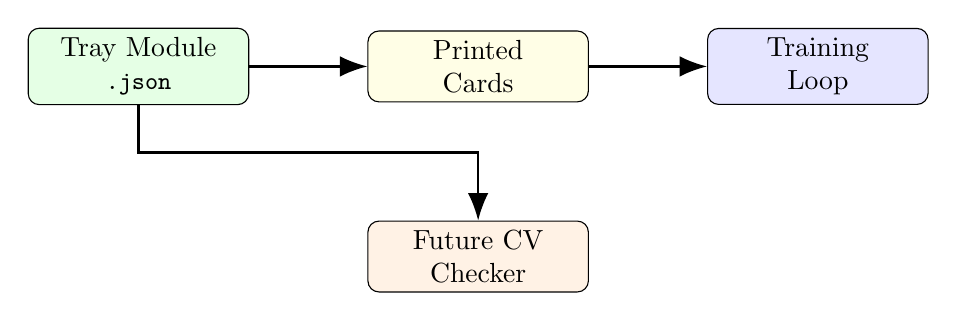
\begin{tikzpicture}[
    node distance=1.5cm,
    box/.style={rectangle, draw, rounded corners, minimum width=2.8cm, minimum height=0.9cm, align=center, fill=blue!10},
    arrow/.style={-{Latex[scale=1.5]}, thick}
  ]
    \node[box, fill=green!10] (module) {Tray Module\\{\small\tt .json}};
    \node[box, right=of module, fill=yellow!10] (cards) {Printed\\Cards};
    \node[box, right=of cards, fill=blue!10] (training) {Training\\Loop};
    \node[box, below=of cards, fill=orange!10] (cv) {Future CV\\Checker};

    \draw[arrow] (module) -- (cards);
    \draw[arrow] (cards) -- (training);
    \draw[arrow] (module.south) -- ++(0,-0.6) -| (cv);
  \end{tikzpicture}
  \vspace{0.5cm}
  \begin{block}{Local knowledge is prerequisite infrastructure}
    The module captures names, aliases, lookalikes, and counts ---
    needed whether you are training now or automating later.
  \end{block}
\end{frame}

% --- Slide 8: Current Status ---------------------------------------------
\begin{frame}{Current Status \& Next Steps}
  \begin{columns}[T]
    \column{0.5\textwidth}
    \textbf{Delivered}
    \begin{itemize}
      \item Problem evidence from published literature
      \item Working web app with 7-step learning loop
      \item 8 file-backed tray modules
      \item Scoring engine with 6 categories
      \item Card generation pipeline
      \item Study protocol with falsification criteria
    \end{itemize}
    \column{0.5\textwidth}
    \textbf{Next step: pilot}
    \begin{itemize}
      \item Baseline pre/post study (8--12 participants)
      \item 7-day retention check
      \item Expert content review
    \end{itemize}
    \vspace{0.3cm}
    \begin{exampleblock}{Seeking partner}
      Hospital or SPD training program to pilot the first module
      with real tray content.
    \end{exampleblock}
  \end{columns}
\end{frame}

\end{document}
